% Provenance (never printed): cycle 4 SVT/physique, "La planete Terre,
% l'environnement": the ocean, its relief, its waters and their movements;
% see sources/book1/PROVENANCE.md. Book 1, grade 8, chapter 4.
% Vocabulary guard: owns the parts of the seafloor (one definition),
% salinity, ocean current (homograph: electric current -- link "ocean
% current" only), gyre. Ridge and trench were met as places in g7.1 (plate
% boundaries); seafloor spreading and subduction stay there. The deep
% circulation is told (no "thermohaline" definition: Book 2).
\chapter{Los océanos}\label{ch:g8:the-oceans}

En diciembre de 1872, un buque de la Marina británica, el HMS
\emph{Challenger}, salió de Inglaterra para un viaje de tres años y medio
alrededor del mundo. Su misión era nueva: averiguar qué hay en el fondo de
los \omterm{def:g2:water-on-earth:ocean}{océanos}. Una y otra vez, el barco se detenía en alta \omterm{def:g2:water-on-earth:ocean}{mar} y la
tripulación bajaba un peso con una larga cuerda hasta que tocaba el fondo;
la longitud de cuerda soltada daba la profundidad. Cuando el barco regresó,
en mayo de 1876, sus sondeos habían mostrado que el fondo del \omterm{def:g2:water-on-earth:ocean}{océano} tiene
\omterm{def:g1:landscapes-around-us:landform}{llanuras} profundas y grandes \omterm{def:g4:world-physical-map:range}{cordilleras}.
% ledger: nhm:challenger-voyage, edin:challenger-stations

\begin{omfigure}
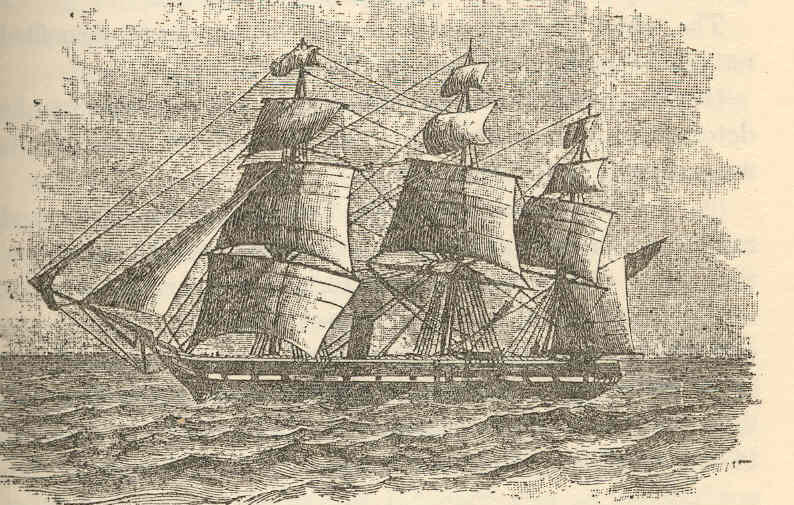
\includegraphics[width=0.55\linewidth]{images/book1/g8-challenger-sounding.jpg}

{\small El HMS \emph{Challenger} preparándose para sondear la profundidad
del \omterm{def:g2:water-on-earth:ocean}{océano}, 1872. Grabado de los informes de la expedición, reproducido en
W.~A.~Herdman, \emph{Founders of Oceanography} (1923); dominio público, vía
Wikimedia Commons.}
% ledger: commons:challenger
\label{fig:g8:the-oceans:challenger}
\end{omfigure}

Hoy un barco cartografía el fondo del \omterm{def:g2:water-on-earth:ocean}{mar} con sonido. Un aparato situado
bajo su casco envía hacia abajo un breve impulso de sonido; el sonido rebota
en el fondo y vuelve en forma de eco. El tiempo que tarda el eco da la
profundidad, una y otra vez, mientras el barco sigue navegando. Es el
\emph{sonar}.
% ledger: nos:sonar

\begin{recall}
El \omterm{def:g2:water-on-earth:salt-fresh}{agua salada} cubre la mayor parte de la Tierra, en un único \omterm{def:g2:water-on-earth:ocean}{océano}
mundial dividido en \omterm{def:g2:water-on-earth:ocean}{océanos} y \omterm{def:g2:water-on-earth:ocean}{mares} (\cref{ch:g2:water-on-earth}). Las
\omterm{def:g7:plate-tectonics:plate}{placas} se separan en las \omterm{def:g8:the-oceans:seafloor}{dorsales oceánicas}, y una \omterm{def:g7:plate-tectonics:plate}{placa} se hunde bajo otra
en las fosas (\cref{ch:g7:plate-tectonics}). Sobre los \omterm{def:g2:water-on-earth:ocean}{océanos}, los vientos
soplan en grandes franjas: \omterm{def:g8:winds-global-circulation:global-winds}{alisios}, \omterm{def:g8:winds-global-circulation:global-winds}{vientos del oeste} y \omterm{def:g8:winds-global-circulation:global-winds}{vientos polares del
este}, desviados por la rotación de la Tierra
(\cref{ch:g8:winds-global-circulation}).
\end{recall}

\section{El fondo del océano}

Si se pudiera vaciar el agua de los \omterm{def:g2:water-on-earth:ocean}{océanos}, aparecería todo un \omterm{def:g1:landscapes-around-us:landscape}{paisaje}
oculto. A lo largo de las \omterm{def:g1:landscapes-around-us:water}{costas}, la tierra continúa bajo el \omterm{def:g2:water-on-earth:ocean}{mar} formando
una plataforma suave y poco profunda. Después el fondo se hunde por una
pendiente empinada hasta unas \omterm{def:g1:landscapes-around-us:landform}{llanuras} inmensas y planas, a kilómetros de
profundidad. De esas \omterm{def:g1:landscapes-around-us:landform}{llanuras} se elevan \omterm{def:g4:world-physical-map:range}{cordilleras}, y aquí y allá unas
fosas estrechas descienden más hondo que cualquier otro lugar de la Tierra.
% ledger: edin:challenger-stations

\begin{omfigure}
\begin{tikzpicture}[font=\footnotesize, >={Stealth[length=2mm]}]
  \fill[omSea] (0,0) rectangle (15.6,-4.2);
  \fill[omLithAlluv] (0,0.6) -- (1.2,0.15) -- (1.6,0) -- (3.4,-0.35)
    .. controls (3.9,-0.55) and (4.1,-2.6) .. (4.7,-3.1)
    -- (6.6,-3.35) -- (7.6,-3.1) -- (8.3,-2.2) -- (8.6,-1.7) -- (8.75,-1.9) -- (8.9,-1.65) -- (9.2,-2.3) -- (10.0,-3.15)
    -- (11.6,-3.4) -- (12.6,-3.45) -- (13.05,-4.1) -- (13.35,-3.0) -- (14.2,-0.9) -- (14.8,0.7) -- (15.6,1.3)
    -- (15.6,-4.6) -- (0,-4.6) -- cycle;
  \draw[black!70] (0,0.6) -- (1.2,0.15) -- (1.6,0) -- (3.4,-0.35)
    .. controls (3.9,-0.55) and (4.1,-2.6) .. (4.7,-3.1)
    -- (6.6,-3.35) -- (7.6,-3.1) -- (8.3,-2.2) -- (8.6,-1.7) -- (8.75,-1.9) -- (8.9,-1.65) -- (9.2,-2.3) -- (10.0,-3.15)
    -- (11.6,-3.4) -- (12.6,-3.45) -- (13.05,-4.1) -- (13.35,-3.0) -- (14.2,-0.9) -- (14.8,0.7) -- (15.6,1.3);
  \draw[omRiver] (1.55,0) -- (14.45,0);
  \node[anchor=south] at (8,0.05) {nivel del mar};
  \node[align=center] at (2.6,-0.85) {plataforma\\continental};
  \draw[->] (2.6,-0.55) -- (2.6,-0.25);
  \node[align=center, anchor=east] at (3.7,-2.0) {talud\\continental};
  \draw[->] (3.75,-2.0) -- (4.1,-1.9);
  \node[align=center] at (5.7,-2.6) {llanura abisal};
  \node[align=center] at (8.75,-0.9) {dorsal oceánica};
  \draw[->] (8.75,-1.15) -- (8.75,-1.55);
  \node[align=center] at (11.1,-2.6) {llanura abisal};
  \node[align=center, anchor=west] at (13.5,-3.9) {fosa\\oceánica};
  \draw[->] (13.45,-3.9) -- (13.15,-3.9);
  \node[anchor=south] at (0.8,0.6) {continente};
  \node[anchor=south east] at (14.7,1.0) {montañas};
\end{tikzpicture}

{\small Las partes del fondo del \omterm{def:g2:water-on-earth:ocean}{océano}, desde una \omterm{def:g1:landscapes-around-us:water}{costa} hasta alta \omterm{def:g2:water-on-earth:ocean}{mar} y
otra \omterm{def:g1:landscapes-around-us:water}{costa} (un esquema: las profundidades y las anchuras no están a
escala).}
\label{fig:g8:the-oceans:sketch}
\end{omfigure}

\begin{definition}[Las partes del fondo del océano]\label{def:g8:the-oceans:seafloor}
\begin{itemize}
  \item La \emph{plataforma continental}\index{plataforma continental} es
        el borde de un \omterm{def:g3:continents-and-oceans:continent}{continente} bajo el \omterm{def:g2:water-on-earth:ocean}{mar}, poco profundo y de pendiente
        suave.
  \item El \emph{talud continental}\index{talud continental} es la
        pendiente empinada que baja desde la plataforma hasta el fondo
        oceánico profundo.
  \item Una \emph{llanura abisal}\index{llanura abisal} es una parte
        inmensa, muy plana y profunda del fondo del \omterm{def:g2:water-on-earth:ocean}{océano}.
  \item Una \emph{dorsal oceánica}\index{dorsal oceanica@dorsal oceánica}
        es una larga cadena de \omterm{def:g1:landscapes-around-us:landform}{montañas} submarinas que se eleva desde las
        \omterm{def:g1:landscapes-around-us:landform}{llanuras} abisales.
  \item Una \emph{fosa oceánica}\index{fosa oceanica@fosa oceánica} es una
        depresión larga, estrecha y muy profunda del fondo del \omterm{def:g2:water-on-earth:ocean}{océano}, a
        menudo junto a una cadena de \omterm{def:g1:landscapes-around-us:landform}{montañas} o de islas volcánicas.
\end{itemize}
\end{definition}
% ledger: edin:challenger-stations, usgs:trench-depth

El \omterm{def:g2:water-on-earth:ocean}{océano} tiene una profundidad media de unos \qty{3700}{m}, casi la mitad
de la altura de la \omterm{def:g1:landscapes-around-us:landform}{montaña} más alta de tierra firme. Su punto más profundo,
el abismo Challenger, en la fosa de las Marianas, en el \omterm{def:g2:water-on-earth:ocean}{océano} Pacífico,
está a casi \qty{11000}{m} por debajo de la superficie.
% ledger: nos:ocean-depth, usgs:trench-depth, tht:everest


\begin{method}[Leer un perfil del fondo del océano]
\begin{enumerate}
  \item Lee los ejes: la distancia en horizontal, la altura o la
        profundidad en vertical, y la exageración vertical.
  \item Busca el \omterm{def:g4:world-physical-map:altitude}{nivel del mar} (altura 0) y las \omterm{def:g1:landscapes-around-us:water}{costas}, donde el perfil lo
        corta.
  \item Sigue el fondo desde una \omterm{def:g1:landscapes-around-us:water}{costa}: la plataforma poco profunda, el
        talud empinado y luego las \omterm{def:g1:landscapes-around-us:landform}{llanuras} profundas y planas.
  \item Busca lo que se eleva sobre las \omterm{def:g1:landscapes-around-us:landform}{llanuras} (una dorsal) o lo que baja
        por debajo de ellas (una fosa), y lee su profundidad.
\end{enumerate}
\end{method}

\begin{example}[A través del Atlántico Sur]
En el perfil de arriba, pasada la \omterm{def:g1:landscapes-around-us:water}{costa} de América del Sur, el fondo baja
a más de \qty{3000}{m} de profundidad en menos de \qty{300}{km}. Unas
\omterm{def:g8:the-oceans:seafloor}{llanuras abisales}, de entre \qty{3500}{m} y \qty{5000}{m} de profundidad,
ocupan la mayor parte de la anchura. A medio camino, a unos
\qty{4400}{km} a lo largo del perfil, la dorsal mesoatlántica se eleva
hasta unos \qty{2300}{m} por debajo de la superficie: más de
\qty{2000}{m} por encima de las \omterm{def:g1:landscapes-around-us:landform}{llanuras}, una \omterm{def:g4:world-physical-map:range}{cordillera} oculta bajo el
\omterm{def:g2:water-on-earth:ocean}{mar}. Las \omterm{def:g1:landscapes-around-us:landform}{llanuras} vuelven a hundirse a más de \qty{5000}{m} antes de que
el fondo suba hacia África.
\end{example}
% ledger: data:etopo1 (figdata/grade-8/seafloor_profile.py: ridge crest -2329 m at 4407 km; deepest -5295 m)

\begin{omfigure}
\begin{tikzpicture}
\begin{axis}[omsection, scale only axis, width=14cm, height=3.6cm, xmin=0, xmax=7569,
  ymin=-6000, ymax=1500, ytick={-6000,-4000,-2000,0}, xtick={0,1000,...,7000},
  xlabel={distancia a lo largo de 30.5\textdegree\ S, desde 59.5\textdegree\ O (km)}, ylabel={altura (m)},
  tick label style={font=\scriptsize}, label style={font=\small},
  yticklabel style={/pgf/number format/1000 sep={\,}}, xticklabel style={/pgf/number format/1000 sep={\,}},
  axis background/.style={fill=white}, clip=true]
  \fill[omSea] (axis cs:0,-6000) rectangle (axis cs:7569,0);
  \addplot[fill=omLithAlluv, draw=black!70, line width=0.5pt] table[x=km, y=elev_m] {figdata/out/grade-8-seafloor_profile-atlantic-rock.dat};
  \node[font=\scriptsize, align=center, fill=white, inner sep=1pt] at (axis cs:4407,-900) {dorsal mesoatlántica};
  \draw[-{Stealth[length=1.5mm]}] (axis cs:4407,-1250) -- (axis cs:4407,-2150);
  \node[font=\scriptsize] at (axis cs:2500,-5300) {llanura abisal};
  \node[font=\scriptsize] at (axis cs:6200,-5600) {llanura abisal};
  \node[font=\scriptsize, anchor=south west] at (axis cs:30,350) {América del Sur};
  \node[font=\scriptsize, anchor=south east] at (axis cs:7380,350) {África};
  \node[anchor=north] at (rel axis cs:0.75,0.97) {\omve{260}};
\end{axis}
\end{tikzpicture}

\medskip
\begin{tikzpicture}
\begin{axis}[omsection, scale only axis, width=7cm, height=3.6cm, xmin=0, xmax=3020,
  ymin=-6000, ymax=4500, ytick={-6000,-4000,-2000,0,2000,4000}, xtick={0,1000,2000,3000},
  xlabel={distancia a lo largo de 20.5\textdegree\ S (km)}, ylabel={altura (m)},
  tick label style={font=\scriptsize}, label style={font=\small},
  yticklabel style={/pgf/number format/1000 sep={\,}}, xticklabel style={/pgf/number format/1000 sep={\,}},
  axis background/.style={fill=white}, clip=true]
  \fill[omSea] (axis cs:0,-6000) rectangle (axis cs:3020,0);
  \addplot[fill=omLithAlluv, draw=black!70, line width=0.5pt] table[x=km, y=elev_m] {figdata/out/grade-8-seafloor_profile-pacific-rock.dat};
  \node[font=\scriptsize, align=center, fill=white, inner sep=1pt] at (axis cs:1300,1600) {fosa de Perú-Chile};
  \draw[-{Stealth[length=1.5mm]}] (axis cs:1750,1150) -- (axis cs:1870,-5000);
  \node[font=\scriptsize, anchor=west] at (axis cs:2600,3500) {Andes};
  \node[font=\scriptsize] at (axis cs:700,-5300) {llanura abisal};
  \node[anchor=north west] at (rel axis cs:0.01,0.98) {\omve{148}};
\end{axis}
\end{tikzpicture}

{\small Dos perfiles reales del fondo del \omterm{def:g2:water-on-earth:ocean}{océano}, a partir del relieve
ETOPO1 leído cada grado de \omterm{def:g6:latitude-longitude:longitude}{longitud}. Arriba: a través del Atlántico Sur, de
América del Sur a África. Abajo: a través del borde pacífico de América del
Sur. Las alturas están multiplicadas por 260 y por 148 respecto a las
distancias (\emph{exageración vertical}); si no, el \omterm{def:g2:water-on-earth:ocean}{océano} parecería tan
fino como una hoja de papel; y con un punto por grado, la estrecha fosa
parece menos profunda de lo que es.}
% ledger: data:etopo1, earth:Rmean (figdata/grade-8/seafloor_profile.py)
\label{fig:g8:the-oceans:profiles}
\end{omfigure}


\section{Un agua salada}

El agua del \omterm{def:g2:water-on-earth:ocean}{mar} sabe salada porque tiene sales disueltas. La mayoría
proceden de las \omterm{def:g3:stones-pebbles-sand:rock}{rocas} de los \omterm{def:g3:continents-and-oceans:continent}{continentes}: la \omterm{def:g4:clouds-rain-snow:precipitation}{lluvia} desgasta lentamente
las \omterm{def:g3:stones-pebbles-sand:rock}{rocas} y los \omterm{def:g1:landscapes-around-us:water}{ríos} llevan sus sales disueltas hasta el \omterm{def:g2:water-on-earth:ocean}{mar}. Algunas
proceden de manantiales calientes del fondo del \omterm{def:g2:water-on-earth:ocean}{océano}.
% ledger: nos:salinity-varies

\begin{definition}[Salinidad]\label{def:g8:the-oceans:salinity}
La \emph{salinidad}\index{salinidad} del agua del \omterm{def:g2:water-on-earth:ocean}{mar} es la masa de sales
disueltas en un kilogramo de agua de \omterm{def:g2:water-on-earth:ocean}{mar}. De media es de unos \qty{35}{g}
por kilogramo: el \qty{3.5}{\%} de la masa del agua de \omterm{def:g2:water-on-earth:ocean}{mar} es sal.
\end{definition}
% ledger: nos:salinity-varies

La \omterm{def:g8:the-oceans:salinity}{salinidad} no es la misma en todas partes. Cuando el agua del \omterm{def:g2:water-on-earth:ocean}{mar} se
evapora, el agua se va pero las sales se quedan: donde el Sol es fuerte y
la \omterm{def:g4:clouds-rain-snow:precipitation}{lluvia} escasa, el \omterm{def:g2:water-on-earth:ocean}{mar} se vuelve más salado. Donde cae mucha \omterm{def:g4:clouds-rain-snow:precipitation}{lluvia}, o
donde desemboca un gran \omterm{def:g1:landscapes-around-us:water}{río}, el \omterm{def:g2:water-on-earth:ocean}{mar} es menos salado. Cuando el agua del \omterm{def:g2:water-on-earth:ocean}{mar}
se congela y forma hielo marino, la sal se queda en el agua de alrededor,
que también se vuelve más salada. En conjunto, la \omterm{def:g8:the-oceans:salinity}{salinidad} es baja cerca
del \omterm{def:g3:continents-and-oceans:equator}{ecuador}, donde llueve mucho, y cerca de los \omterm{def:g3:continents-and-oceans:poles}{polos}; es máxima en las
\omterm{def:g6:latitude-longitude:latitude}{latitudes} medias, bajo las franjas secas de los \ang{30}.
% ledger: nos:salinity-varies, nos:sea-ice-salt, mo:three-cells

\begin{omfigure}
\begin{tikzpicture}[font=\footnotesize, >={Stealth[length=2mm]}]
  \fill[omSea] (0,0) rectangle (13,-1.6);
  \draw[omRiver, line width=0.8pt] (0,0) -- (13,0);
  % left: dry belt, evaporation
  \fill[yellow!80!orange] (1.2,3.0) circle (0.35);
  \foreach \x in {1.0,1.8,2.6,3.4} \draw[->, black!50, line width=0.9pt, decorate, decoration={snake, amplitude=0.6mm, segment length=3mm}] (\x,0.15) -- (\x,1.6);
  \node[align=center] at (2.3,2.2) {mucha evaporación,\\poca lluvia};
  \node[align=center, fill=white, inner sep=1.5pt] at (2.3,-0.8) {\textbf{más salada}};
  % middle: rain
  \fill[black!20] (5.2,2.9) ellipse [x radius=1.3, y radius=0.4];
  \foreach \x in {4.4,4.8,...,6.0} \draw[omRiver] (\x,2.45) -- (\x-0.2,0.25);
  \node[align=center, fill=white, inner sep=1.5pt] at (5.2,-0.8) {\textbf{menos salada}};
  \node at (5.2,3.55) {lluvia intensa};
  % right: river mouth and sea ice
  \fill[omLithAlluv] (7.4,0) -- (9.6,0) -- (9.6,0.6) -- (7.4,0.35) -- cycle;
  \draw[omRiver, line width=2pt, ->] (9.4,0.45) -- (7.9,0.2);
  \node[anchor=south] at (8.6,0.65) {río};
  \node[align=center, fill=white, inner sep=1.5pt] at (8.6,-0.8) {\textbf{menos salada}};
  \fill[white, draw=omCold] (10.6,0.25) -- (12.6,0.25) -- (12.4,-0.25) -- (10.8,-0.25) -- cycle;
  \node[anchor=south] at (11.6,0.3) {se forma hielo marino};
  \node[align=center, fill=white, inner sep=1.5pt] at (11.6,-0.95) {\textbf{más salada}\\(la sal se queda)};
\end{tikzpicture}

{\small Lo que cambia la \omterm{def:g8:the-oceans:salinity}{salinidad} del \omterm{def:g2:water-on-earth:ocean}{mar}: la evaporación y la congelación
dejan atrás las sales; la \omterm{def:g4:clouds-rain-snow:precipitation}{lluvia} y los \omterm{def:g1:landscapes-around-us:water}{ríos} aportan \omterm{def:g2:water-on-earth:salt-fresh}{agua dulce}.}
% ledger: nos:salinity-varies, nos:sea-ice-salt
\label{fig:g8:the-oceans:salinity}
\end{omfigure}

\begin{omfigure}
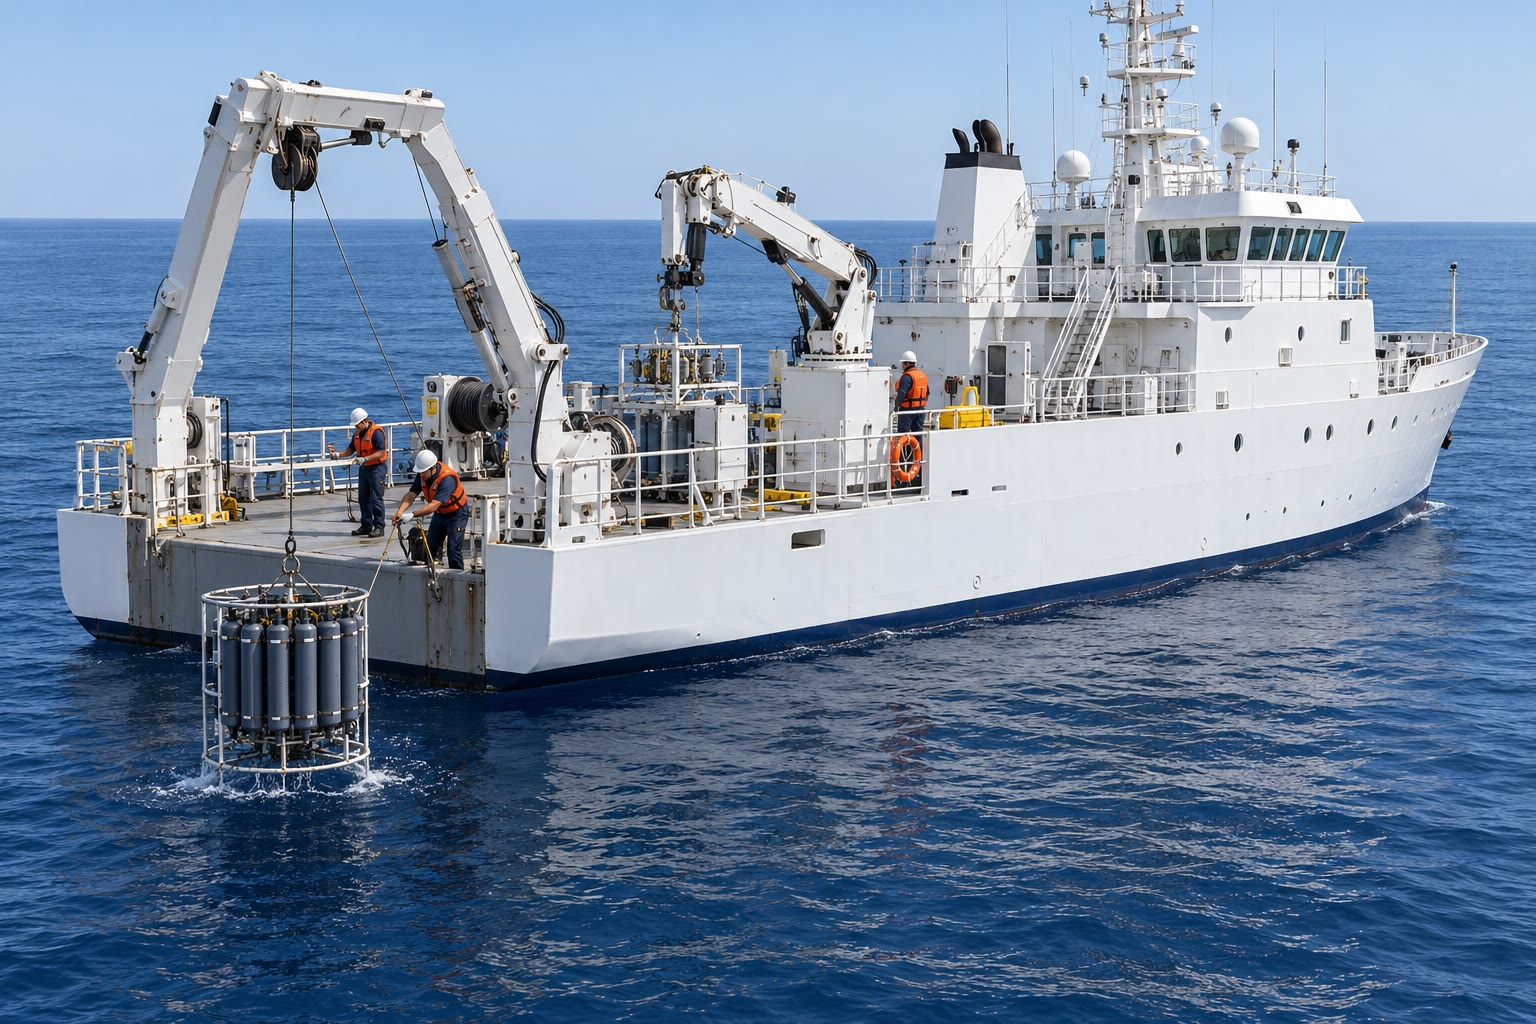
\includegraphics[width=0.58\linewidth]{images/book1/ai/g8-research-ship.jpg}

{\small Un buque oceanográfico baja al \omterm{def:g2:water-on-earth:ocean}{mar} un bastidor con botellas de
muestreo, para traer agua de las profundidades y medir su \omterm{def:g8:the-oceans:salinity}{salinidad} y su
temperatura (ilustración generada por IA de una escena genérica).}
\label{fig:g8:the-oceans:ship}
\end{omfigure}

\section{Las corrientes de superficie}

El \omterm{def:g2:water-on-earth:ocean}{océano} nunca está quieto. Los vientos arrastran su superficie y ponen el
agua en movimiento: los \omterm{def:g8:winds-global-circulation:global-winds}{alisios}, constantes, la empujan hacia el oeste
cerca del \omterm{def:g3:continents-and-oceans:equator}{ecuador}, y los \omterm{def:g8:winds-global-circulation:global-winds}{vientos del oeste} la empujan hacia el este en las
\omterm{def:g6:latitude-longitude:latitude}{latitudes} medias. Como los vientos, el agua en movimiento se desvía por la
rotación de la Tierra: hacia la derecha en el \omterm{def:g3:continents-and-oceans:equator}{hemisferio norte} y hacia la
izquierda en el \omterm{def:g3:continents-and-oceans:equator}{hemisferio sur}.
% ledger: nos:gyres

\begin{definition}[Corriente oceánica y giro oceánico]\label{def:g8:the-oceans:current}
Una \emph{corriente oceánica}\index{corriente oceanica@corriente oceánica}
es un movimiento constante del agua del \omterm{def:g2:water-on-earth:ocean}{mar} en una dirección, como un \omterm{def:g1:landscapes-around-us:water}{río}
dentro del \omterm{def:g2:water-on-earth:ocean}{océano}. Un \emph{giro oceánico}\index{giro oceanico@giro oceánico}
es un circuito muy grande de corrientes oceánicas que gira alrededor de
una cuenca oceánica.
\end{definition}
% ledger: nos:gyre-def, nos:gyres
\phantomsection\label{def:g8:the-oceans:gyre}

Hay cinco grandes \omterm{def:g8:the-oceans:current}{giros}: en el Atlántico Norte y Sur, en el Pacífico Norte
y Sur, y en el \omterm{def:g2:water-on-earth:ocean}{océano} Índico. Los del \omterm{def:g3:continents-and-oceans:equator}{hemisferio norte} giran en el sentido
de las agujas del reloj, y los del \omterm{def:g3:continents-and-oceans:equator}{hemisferio sur}, en sentido contrario. En
el lado occidental de cada \omterm{def:g2:water-on-earth:ocean}{océano}, la corriente del \omterm{def:g8:the-oceans:current}{giro} es estrecha y
rápida; en el lado oriental, es ancha y lenta.
% ledger: nos:gyres

\begin{inthelab}[Un giro en una fuente]
En el interior, llena de agua una fuente redonda grande y espolvorea una
pizca de pimienta sobre la superficie. Sopla con suavidad y sin parar a
través de una pajita, siempre en la misma dirección, cerca de un borde.
Observa la pimienta: el agua de la superficie empieza a moverse con tu
soplo, y pronto toda la superficie gira en un circuito alrededor de la
fuente.
\end{inthelab}

\begin{omfigure}
\begin{tikzpicture}
\begin{axis}[ommap, width=\linewidth, xmin=-180, xmax=180, ymin=-65, ymax=70,
  xtick={-180,-120,...,180}, ytick={-60,-30,0,30,60},
  xticklabels={$180^\circ$,$120^\circ$O,$60^\circ$O,$0^\circ$,$60^\circ$E,$120^\circ$E,$180^\circ$},
  yticklabels={$60^\circ$S,$30^\circ$S,$0^\circ$,$30^\circ$N,$60^\circ$N},
  tick label style={font=\scriptsize}]
  \addplot[fill=omLithAlluv, draw=black!45, line width=0.2pt] table {figdata/out/shared-geo-land.dat};
  \addplot[omWarm, line width=1.3pt] table {figdata/out/grade-8-ocean_currents-gyres-warm.dat};
  \addplot[omCold, line width=1.3pt] table {figdata/out/grade-8-ocean_currents-gyres-cold.dat};
  \addplot[quiver={u=\thisrow{u}, v=\thisrow{v}}, -{Stealth[length=2.6mm, width=2.2mm]}, omWarm, line width=1.3pt]
    table[x=lon, y=lat] {figdata/out/grade-8-ocean_currents-heads-warm.dat};
  \addplot[quiver={u=\thisrow{u}, v=\thisrow{v}}, -{Stealth[length=2.6mm, width=2.2mm]}, omCold, line width=1.3pt]
    table[x=lon, y=lat] {figdata/out/grade-8-ocean_currents-heads-cold.dat};
  \node[font=\scriptsize\bfseries, fill=white, inner sep=1pt, anchor=east] at (axis cs:-72,40) {corriente del Golfo};
  \node[font=\scriptsize\bfseries, fill=white, inner sep=1pt, anchor=west] at (axis cs:-12,25) {C. de Canarias};
\end{axis}
\end{tikzpicture}

{\small Los cinco grandes \omterm{def:g8:the-oceans:current}{giros}, simplificados: en el sentido de las agujas
del reloj en el \omterm{def:g3:continents-and-oceans:equator}{hemisferio norte}, en sentido contrario en el sur. En rojo:
corrientes cálidas, que vienen de los \omterm{def:g5:weather-and-climate:tropics}{trópicos}; en azul: corrientes frías,
que vienen de \omterm{def:g6:latitude-longitude:latitude}{latitudes} más altas. El \omterm{def:g8:the-oceans:current}{giro} del Atlántico Norte está
bordeado por la corriente del Golfo al oeste y por la corriente de Canarias
al este.}
% ledger: nos:gyres, data:ne-land (figdata/grade-8/ocean_currents.py)
\label{fig:g8:the-oceans:gyres}
\end{omfigure}

La más conocida de estas corrientes es la corriente del Golfo. Sale del
golfo de México, sube hacia el norte a lo largo de la \omterm{def:g1:landscapes-around-us:water}{costa} de Florida,
gira hacia el este frente a Carolina del Norte y cruza el Atlántico hacia
el nordeste. Su agua cálida se desplaza de media a unos \qty{6.4}{km} por
hora, hasta unos \qty{9}{km} por hora en la superficie, y transporta más
agua que todos los \omterm{def:g1:landscapes-around-us:water}{ríos} del mundo juntos. Mantiene más templada en invierno
la \omterm{def:g1:landscapes-around-us:water}{costa} este de Florida y lleva aire suave a Europa occidental.
% ledger: nos:gulf-stream, nos:gyres

\begin{omfigure}
\begin{minipage}[c]{0.5\linewidth}\centering
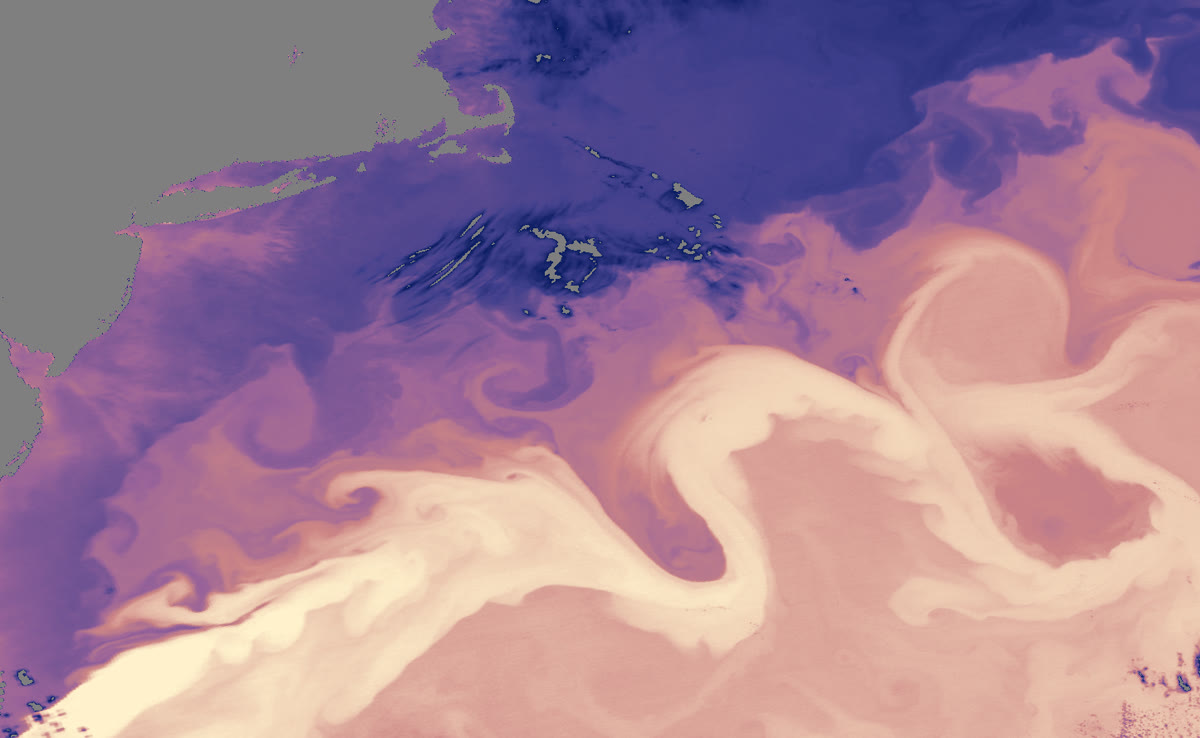
\includegraphics[width=\linewidth]{images/book1/g8-gulf-stream-sst.jpg}
\end{minipage}\hfill
\begin{minipage}[c]{0.46\linewidth}\raggedright
{\small La temperatura de la superficie del \omterm{def:g2:water-on-earth:ocean}{mar} frente a la \omterm{def:g1:landscapes-around-us:water}{costa} este de
América del Norte, medida por el satélite Aqua de la NASA el 18~de abril de
2005. La corriente del Golfo es la franja de agua cálida (colores claros,
hasta unos \qty{23}{\degreeCelsius}) que serpentea desde abajo a la
izquierda hacia la derecha, entre aguas más frías (oscuras, hasta unos
\qty{-1}{\degreeCelsius}); la tierra está en gris. NASA (dominio público,
vía Wikimedia Commons).}
\end{minipage}
% ledger: commons:gulf-sst
\label{fig:g8:the-oceans:gulf}
\end{omfigure}


\section{Las corrientes profundas y el calor del océano}

Los vientos mueven las corrientes de superficie. Muy por debajo, en la
oscuridad fría del \omterm{def:g2:water-on-earth:ocean}{océano} profundo, el agua también se mueve, mucho más
despacio. En el extremo norte del Atlántico, el agua cálida que trae la
corriente del Golfo cede su calor al aire frío; enfriada, y más salada
cuando se forma el hielo marino, se vuelve más densa y se hunde hasta el
fondo. Esta agua fría y salada avanza lentamente hacia el sur a ras del
fondo oceánico, hasta la Antártida, y después hacia los \omterm{def:g2:water-on-earth:ocean}{océanos} Índico y
Pacífico, donde sube poco a poco y vuelve a la superficie. Una gota de agua
puede tardar unos \num{1000} años en dar una vuelta a este gran circuito,
la \emph{cinta transportadora oceánica global}.
% ledger: nos:conveyor, nos:sea-ice-salt

\begin{omfigure}
\begin{tikzpicture}
\begin{axis}[ommap, width=\linewidth, xmin=-180, xmax=180, ymin=-65, ymax=70,
  xtick={-180,-120,...,180}, ytick={-60,-30,0,30,60},
  xticklabels={$180^\circ$,$120^\circ$O,$60^\circ$O,$0^\circ$,$60^\circ$E,$120^\circ$E,$180^\circ$},
  yticklabels={$60^\circ$S,$30^\circ$S,$0^\circ$,$30^\circ$N,$60^\circ$N},
  tick label style={font=\scriptsize}]
  \addplot[fill=omLithAlluv, draw=black!45, line width=0.2pt] table {figdata/out/shared-geo-land.dat};
  \addplot[omWarm, line width=1.3pt] table {figdata/out/grade-8-conveyor-surface.dat};
  \addplot[omCold, line width=1.3pt, dashed] table {figdata/out/grade-8-conveyor-deep.dat};
  \addplot[quiver={u=\thisrow{u}, v=\thisrow{v}}, -{Stealth[length=2.6mm, width=2.2mm]}, omWarm, line width=1.3pt]
    table[x=lon, y=lat] {figdata/out/grade-8-conveyor-heads-surface.dat};
  \addplot[quiver={u=\thisrow{u}, v=\thisrow{v}}, -{Stealth[length=2.6mm, width=2.2mm]}, omCold, line width=1.3pt]
    table[x=lon, y=lat] {figdata/out/grade-8-conveyor-heads-deep.dat};
  \node[font=\scriptsize\bfseries, fill=white, inner sep=1pt, anchor=west] at (axis cs:4,64) {se hunde};
  \node[font=\scriptsize\bfseries, fill=white, inner sep=1pt, anchor=south] at (axis cs:163,11) {sube};
\end{axis}
\end{tikzpicture}

{\small La cinta transportadora oceánica global, simplificada en un solo
circuito (un esquema). En rojo: agua cálida en la superficie; en azul,
discontinuo: agua fría y salada que avanza lentamente a ras del fondo
oceánico. El agua se hunde en el extremo norte del Atlántico, entre
Groenlandia y Noruega, y sube en el Pacífico (y, sin dibujar, en el \omterm{def:g2:water-on-earth:ocean}{océano}
Índico).}
% ledger: nos:conveyor, data:ne-land (figdata/grade-8/conveyor.py)
\end{omfigure}

\begin{example}[¿Qué lenta es el agua profunda?]\label{ex:g8:the-oceans:deep-speed}
El circuito dibujado en el \omterm{def:g2:drawing-to-map:map}{mapa} mide aproximadamente \qty{70000}{km}. Si
una gota de agua tarda unos \num{1000} años en recorrerlo, se desplaza de
media unos $\num{70000} \div \num{1000} = \qty{70}{km}$ al año, es decir,
unos \qty{200}{m} al día. La corriente del Golfo, a \qty{6.4}{km} por
hora, recorre unos \qty{150}{km} en un día: llega tan lejos en unas 11
horas como el agua profunda en todo un año.
% ledger: nos:conveyor, nos:gulf-stream, earth:Rmean (loop length and speeds computed in figdata/grade-8/conveyor.py)
\end{example}

Juntas, las corrientes de superficie y las profundas transportan calor: el
agua cálida va de los \omterm{def:g5:weather-and-climate:tropics}{trópicos} hacia los \omterm{def:g3:continents-and-oceans:poles}{polos}, y el agua fría vuelve hacia
el \omterm{def:g3:continents-and-oceans:equator}{ecuador}. Como los vientos, el \omterm{def:g2:water-on-earth:ocean}{océano} compensa el calentamiento desigual
de la Tierra por el Sol.
% ledger: nos:conveyor, nos:gulf-stream, mo:global-circ

\section{Ejercicios}

\begin{exercise}[$\star$]\label{exo:g8:the-oceans:1}
Ordena estas partes del fondo del \omterm{def:g2:water-on-earth:ocean}{océano} tal como las encuentra un
submarino que sale de una \omterm{def:g1:landscapes-around-us:water}{costa} hacia el centro del Atlántico: \omterm{def:g8:the-oceans:seafloor}{llanura
abisal}; \omterm{def:g8:the-oceans:seafloor}{talud continental}; \omterm{def:g8:the-oceans:seafloor}{dorsal oceánica}; \omterm{def:g8:the-oceans:seafloor}{plataforma continental}.
\end{exercise}

\begin{exercise}[$\star$]\label{exo:g8:the-oceans:2}
¿Verdadero o falso? Corrige las frases falsas. (a) El \omterm{def:g2:water-on-earth:ocean}{océano} tiene una
profundidad media de unos \qty{37}{km}. (b) Los \omterm{def:g8:the-oceans:current}{giros} del \omterm{def:g3:continents-and-oceans:equator}{hemisferio norte}
giran en el sentido de las agujas del reloj. (c) La evaporación hace que el
agua del \omterm{def:g2:water-on-earth:ocean}{mar} sea menos salada. (d) La corriente del Golfo es una corriente
cálida.
\end{exercise}

\begin{exercise}[$\star$]\label{exo:g8:the-oceans:3}
Da la palabra que corresponde a cada descripción: (a) una larga cadena de
\omterm{def:g1:landscapes-around-us:landform}{montañas} bajo el \omterm{def:g2:water-on-earth:ocean}{mar}; (b) la masa de sal que hay en un kilogramo de agua de
\omterm{def:g2:water-on-earth:ocean}{mar}; (c) un circuito muy grande de \omterm{def:g8:the-oceans:current}{corrientes oceánicas}; (d) una depresión
larga, estrecha y muy profunda del fondo del \omterm{def:g2:water-on-earth:ocean}{océano}.
\end{exercise}

\begin{exercise}[$\star$]\label{exo:g8:the-oceans:4}
En el \omterm{def:g2:drawing-to-map:map}{mapa} de los \omterm{def:g8:the-oceans:current}{giros}: (a) ¿en qué sentido gira el \omterm{def:g8:the-oceans:current}{giro} del Atlántico
Sur? (b) Nombra una corriente cálida y una corriente fría del Atlántico
Norte. (c) ¿Qué vientos empujan el agua hacia el oeste cerca del \omterm{def:g3:continents-and-oceans:equator}{ecuador}?
\end{exercise}

\begin{exercise}[$\star\star$]\label{exo:g8:the-oceans:5}
Una muestra de \qty{1}{kg} de agua de \omterm{def:g2:water-on-earth:ocean}{mar} contiene \qty{35}{g} de sales.
(a) ¿Qué porcentaje de su masa es sal? (b) ¿Cuántos gramos de sales hay en
\qty{20}{kg} de esta agua? (c) ¿Cuántos kilogramos de agua de \omterm{def:g2:water-on-earth:ocean}{mar} contienen
\qty{1}{kg} de sales?
\end{exercise}

\begin{exercise}[$\star\star$]\label{exo:g8:the-oceans:6}
El sonar de un barco envía un impulso de sonido en vertical hacia abajo. El
eco vuelve \qty{6}{s} después. En el agua de \omterm{def:g2:water-on-earth:ocean}{mar}, el sonido recorre unos
\qty{1500}{m} cada segundo. (a) ¿Qué distancia recorre el sonido en
\qty{6}{s}? (b) ¿Por qué la profundidad es solo la mitad de esa distancia?
(c) ¿Cuál es la profundidad? (d) ¿Sobre qué parte del fondo del \omterm{def:g2:water-on-earth:ocean}{océano}
podría estar el barco?
\end{exercise}

\begin{exercise}[$\star\star$]\label{exo:g8:the-oceans:7}
Usa el perfil a través del Atlántico Sur. (a) ¿Qué profundidad tienen, más
o menos, las \omterm{def:g8:the-oceans:seafloor}{llanuras abisales}? (b) ¿A qué distancia a lo largo del perfil
está la cresta de la dorsal mesoatlántica, y a qué profundidad? (c) ¿Cuántos
metros se eleva la dorsal sobre las \omterm{def:g1:landscapes-around-us:landform}{llanuras}? (d) ¿Por qué el perfil
necesita una exageración vertical?
\end{exercise}

\begin{exercise}[$\star\star$]\label{exo:g8:the-oceans:8}
El \omterm{def:g2:water-on-earth:ocean}{mar} A está entre dos \omterm{def:g5:weather-and-climate:desert}{desiertos}: casi nunca llueve y no desemboca en él
ningún gran \omterm{def:g1:landscapes-around-us:water}{río}. El \omterm{def:g2:water-on-earth:ocean}{mar} B, en una región lluviosa, recibe muchos \omterm{def:g1:landscapes-around-us:water}{ríos}
grandes. Explica cuál de los dos es más salado que el \omterm{def:g2:water-on-earth:ocean}{océano} abierto y cuál
es menos salado. Usa las palabras \emph{evaporación}, \emph{\omterm{def:g2:water-on-earth:salt-fresh}{agua dulce}},
\emph{las sales se quedan}.
\end{exercise}

\begin{exercise}[$\star\star$]\label{exo:g8:the-oceans:9}
Se lanza al \omterm{def:g2:water-on-earth:ocean}{mar} un mensaje en una botella frente a la \omterm{def:g1:landscapes-around-us:water}{costa} de Florida.
(a) ¿Qué corriente lo arrastra primero, y en qué dirección? (b) ¿Hacia
dónde cruza después el Atlántico? (c) Si siguiera dando la vuelta al \omterm{def:g8:the-oceans:current}{giro},
¿a lo largo de qué \omterm{def:g1:landscapes-around-us:water}{costa} viajaría hacia el sur? (d) ¿Es cálida o fría esa
corriente?
\end{exercise}

\begin{exercise}[$\star\star$]\label{exo:g8:the-oceans:10}
La corriente del Golfo se desplaza de media a unos \qty{6.4}{km} por hora.
(a) ¿Qué distancia recorre su agua en un día? (b) ¿Y en una semana?
(c) Compárala con una persona que camina a \qty{5}{km} por hora.
\end{exercise}

\begin{exercise}[$\star\star\star$]\label{exo:g8:the-oceans:11}
El \omterm{def:g2:water-on-earth:ocean}{océano} tiene una profundidad media de unos \qty{3700}{m}, y su punto más
profundo está a casi \qty{11000}{m}. (a) Escribe las dos profundidades en
kilómetros. (b) ¿Cuántas veces más profundo que la media es el punto más
profundo? Redondea a un decimal. (c) Un eco de sonar desde el punto más
profundo: ¿cuántos segundos tarda en volver, a \qty{1500}{m} por segundo?
(d) Una gota de agua de la cinta transportadora se hunde en el Atlántico
Norte. Si tarda unos \num{1000} años en dar la vuelta, ¿cuántos años es
eso en potencias de diez?
\end{exercise}

\begin{exercise}[$\star\star\star$]\label{exo:g8:the-oceans:12}
La gran cinta transportadora del \omterm{def:g2:water-on-earth:ocean}{océano} profundo empieza en el \omterm{def:g2:water-on-earth:ocean}{mar} de
Noruega, frente a la \omterm{def:g1:landscapes-around-us:water}{costa} de Noruega, donde el agua cálida traída por la
corriente del Golfo cede su calor al aire frío. (a) Con el \omterm{def:g2:drawing-to-map:map}{mapa} de los
\omterm{def:g8:the-oceans:current}{giros} y el capítulo, explica paso a paso cómo llegó hasta allí esta agua
cálida desde los \omterm{def:g5:weather-and-climate:tropics}{trópicos}, y qué vientos la empujaron. (b) Explica por qué
el agua se hunde después. (c) ¿Adónde va a continuación?
\end{exercise}

\section{Problema: una boya a la deriva}

\begin{problem}[{Problema de fin de semana --- se lanza una boya a la
deriva frente a Florida y el giro del Atlántico Norte la arrastra; se sigue
su viaje tramo a tramo y se calcula el tiempo que tarda en dar una vuelta}]
\label{pb:g8:the-oceans:1}
% ledger: nos:drifter, nos:gulf-stream, nos:gyres (figdata/grade-8/ocean_currents.py; the leg lengths are rounded, the speeds of legs B to D are exercise data)
Unos científicos lanzan una boya a la deriva frente a la \omterm{def:g1:landscapes-around-us:water}{costa} de Florida.
Flota justo por debajo de la superficie, se mueve con las corrientes y
envía su posición a un satélite. Sus baterías duran alrededor de un año. El
\omterm{def:g2:drawing-to-map:map}{mapa} muestra los cuatro tramos de su viaje alrededor del \omterm{def:g8:the-oceans:current}{giro} del
Atlántico Norte.

\begin{center}
\begin{tikzpicture}
\begin{axis}[ommap, width=11.5cm, xmin=-95, xmax=0, ymin=5, ymax=55,
  xtick={-90,-60,-30,0}, ytick={10,30,50},
  xticklabels={$90^\circ$O,$60^\circ$O,$30^\circ$O,$0^\circ$},
  yticklabels={$10^\circ$N,$30^\circ$N,$50^\circ$N},
  tick label style={font=\scriptsize}]
  \addplot[fill=omLithAlluv, draw=black!45, line width=0.2pt] table {figdata/out/shared-geo-land.dat};
  \addplot[black, line width=1pt, densely dashed, postaction={decorate, decoration={markings,
      mark=between positions 0.04 and 0.98 step 0.08 with {\arrow{Stealth[length=2mm]}}}}]
    table[x=lon, y=lat] {figdata/out/grade-8-ocean_currents-buoy.dat};
  \addplot[only marks, mark=*, mark size=2.2pt, omDef] coordinates {(-79.5,26)};
  \node[font=\scriptsize\bfseries, anchor=east, fill=white, inner sep=1pt] at (axis cs:-81,26) {lanzamiento};
  \addplot[only marks, mark=none, nodes near coords, point meta=explicit symbolic,
    every node near coord/.style={anchor=center, font=\footnotesize\bfseries, circle, fill=white, draw, inner sep=1pt}]
    table[x=lon, y=lat, meta=name] {figdata/out/grade-8-ocean_currents-buoy-legs.dat};
\end{axis}
\end{tikzpicture}

\medskip
{\small
\begin{tabular}{|c|l|c|c|}
\hline
tramo & corriente & longitud (km) & velocidad media (km al día) \\
\hline
A & corriente del Golfo & 3800 & 100 \\
B & corriente del Atlántico Norte & 2100 & 20 \\
C & corriente de Canarias & 3100 & 20 \\
D & corriente norecuatorial & 6100 & 20 \\
\hline
\end{tabular}}
\end{center}

\noindent\textbf{Parte I --- El lanzamiento.}\par\nopagebreak
\begin{enumerate}[beginpenalty=10000]
  \item ¿En qué \omterm{def:g2:water-on-earth:ocean}{océano}, y en qué \omterm{def:g3:continents-and-oceans:equator}{hemisferio}, se lanza la boya?
  \item ¿En qué sentido gira el \omterm{def:g8:the-oceans:current}{giro}? ¿Arrastra a la boya primero hacia el
        norte o hacia el sur?
  \item ¿Es cálida o fría el agua del tramo A? ¿Y la del tramo C? Explícalo.
  \item ¿Qué vientos impulsan las corrientes del tramo B? ¿Y del tramo D?
\end{enumerate}

\noindent\textbf{Parte II --- Alrededor del giro.}\par\nopagebreak
\begin{enumerate}[resume, beginpenalty=10000]
  \item ¿Cuántos días dura el tramo A?
  \item ¿Cuántos días duran los tramos B, C y D?
  \item ¿Cuál es la longitud total del viaje alrededor del \omterm{def:g8:the-oceans:current}{giro}?
  \item ¿Por qué el tramo A es mucho más rápido que los demás?
\end{enumerate}

\noindent\textbf{Parte III --- La duración del viaje.}\par\nopagebreak
\begin{enumerate}[resume, beginpenalty=10000]
  \item ¿Cuántos días necesita la boya para dar una vuelta al \omterm{def:g8:the-oceans:current}{giro}?
  \item Contando un mes como 30 días, ¿cuántos meses son? Redondea al mes
        entero más cercano.
  \item ¿En qué tramo se agotarán las baterías, al cabo de alrededor de un
        año (365 días)?
  \item ¿Cuántos meses más de batería necesitaría la boya para enviar su
        posición durante toda la vuelta?
\end{enumerate}
\end{problem}
